%hello.tex 
\documentclass[twocolumn]{article}
\usepackage{graphicx}
\usepackage{sidecap}
\usepackage{epstopdf}

\begin{document}
\title{How to Structure a \LaTeX{} Document}
\author{Alex Kiar\\Department of Physics\\Western University \\ \texttt{akiar@uwo.ca}}
\date{\today}
\maketitle

\begin{abstract}
Space-based astronomical observatories generate vast quantities of data, and efficient means of analyzing those data are needed. The purpose of this research is to apply machine-learning methods to classification of point sources of light emission in nearby galaxies. An object�s light emission over different wavelengths is the key data for classification as it indicates the composition of the object, along with its other physical attributes. The mean-shift, k-means, and minimum spanning tree clustering methods were applied to observations of point sources in the M83 galaxy, to identify objects that emit similar combinations of light over multiple wavelength bands. The data was collected by the Wide Field Camera 3 on the Hubble Space Telescope. To identify which combination of bands was the best at separating different classes of objects, the strength of the clustering was tested using a silhouette score. This metric measures an object�s distance from a cluster outside the one it was originally assigned to. The clustering results were also compared with the results of independent classification, to determine if each object was correctly identified. The results of this work will allow astronomers to plan observations that can be used to automatically classify objects in nearby galaxies, leading to a stronger understanding of how stars, and star clusters, form and evolve. 
\end{abstract}

\tableofcontents

\section{Introduction}
Introduction to galactic astronomy and clustering methods. 
\subsection{Galactic Astronomy} 
Describe the main features of galaxies. 
\subsection{Clustering}
Describe at a high level what clustering is. 

\section{Data} 
\subsection{WFC3 Survey}
Describe the survey.
\subsection{Preprocessing}
Describe the filters applied to the data.

\begin{figure}[h]
 \centering
 \caption{Uncertaintiy}
 \includegraphics[width=0.5\textwidth]{uncertainty_mag3_225}
\end{figure}

\section{Methods}
\subsection{Meanshift}
Describe meanshift clustering. 

\subsection{DBSCAN}
Describe DBscan clustering. 

\subsection{Affinity Propagation}
Describe Affinity Propagation clustering. 

\subsection{KMeans} 
Describe kmeans clustering. \\
\begin{tabular}{c || c | c}
\hline
Number of Clusters & Bandwidth & Score \\
\hline
3 & 6 & 3 \\ \hline
4 & 65 & 4 \\ \hline
5 & 7 & 8 \\
\hline
\end{tabular}
\\
\begin{figure}[h]
 \centering
 \caption{Kmeans Clustering}
 \includegraphics[width=0.5\textwidth]{xy_7cl_mag05_555-mag05_336vsmag05_814-mag05_657}
\end{figure}
\\
\begin{figure}[h]
 \centering
 \caption{MeanShift Clustering}
 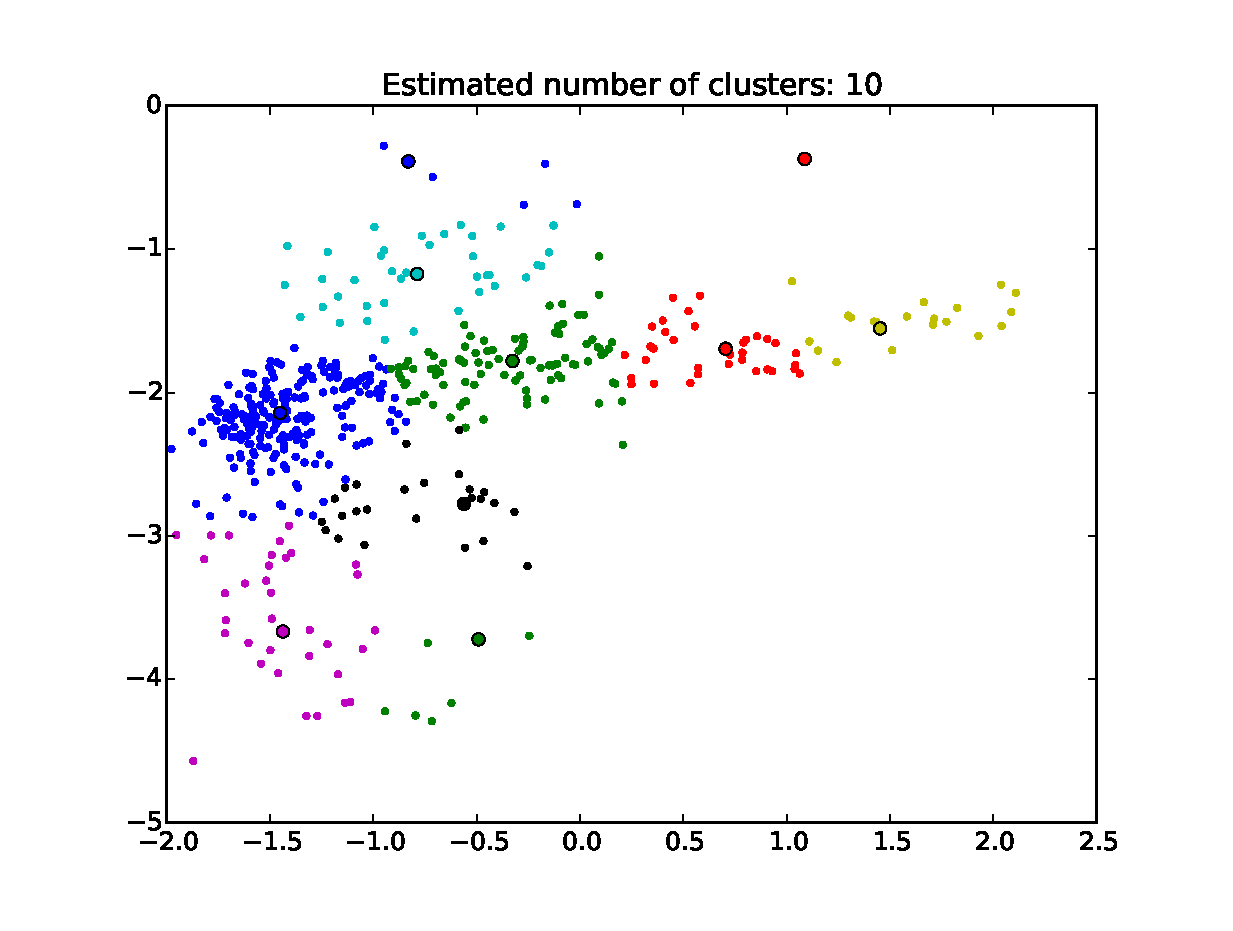
\includegraphics[width=0.5\textwidth]{meanshift_test_336-555vs657-814}
\end{figure}

\section{Results}
What did you learn. 
\begin{enumerate}
\item Silhouette Score
\item Bandwidth
\item Clustering Variability
\item classification
\end{enumerate}

\end{document}